% !TEX program = xelatex
% ══════════════════════════════════════════════════════════════════════════
% MASTER SUPERSET CV — contains ALL confirmed content + impact metrics.
% Tailor by CUTTING from this into applications/<bucket>/<role>/cv.tex.
% This master intentionally runs long (>3 pages) — that is the point.
% PLACEHOLDER CONTENT: this file ships with a fictional example CV so you can
% see the layout in action. Replace every line below with your own — see
% README.md "First-time setup" — but KEEP the preamble/macros/layout as-is.
% ══════════════════════════════════════════════════════════════════════════
\documentclass[9pt]{extarticle}

\usepackage[a4paper,top=6.5mm,bottom=10mm,left=13mm,right=13mm]{geometry}
\usepackage{fontspec}
\usepackage{xcolor}
\usepackage{enumitem}
\usepackage{tikz}
\usepackage{hyperref}
\usepackage{graphicx}
\graphicspath{{../assets/}}
\usepackage{tabularx}
\usepackage{setspace}
\usepackage{needspace}
\usepackage{colortbl}
\usepackage{array}

% ── FONTS (system Avenir Next, matches cv.html) ─────────────
\setmainfont{Avenir Next}[
  UprightFont = * Regular,
  ItalicFont = * Italic,
  BoldFont = * Demi Bold,
  BoldItalicFont = * Demi Bold Italic,
]
% ── Avenir Next weights (Italic variants included where available) ──
\newfontfamily\avenirnextreg{Avenir Next}[
  UprightFont = * Regular,
  ItalicFont = * Italic,
  BoldFont = * Demi Bold,
]
\newfontfamily\avenir{Avenir Next}
\newfontfamily\avenirultralight{Avenir Next}[UprightFont = * Ultra Light, ItalicFont = * Ultra Light Italic]
\newfontfamily\avenirmedium{Avenir Next}[UprightFont = * Medium, ItalicFont = * Medium Italic]
\newfontfamily\avenirdemibold{Avenir Next}[UprightFont = * Demi Bold, ItalicFont = * Demi Bold Italic]
\newfontfamily\avenirbold{Avenir Next}[UprightFont = * Bold, ItalicFont = * Bold Italic]
\newfontfamily\avenirheavy{Avenir Next}[UprightFont = * Heavy, ItalicFont = * Heavy Italic]

% ── Avenir (non-Next) weights (Oblique = its italic style) ──────────
\newfontfamily\avenirlight{Avenir}[UprightFont = * Light, ItalicFont = * Light Oblique]
\newfontfamily\avenirbook{Avenir}[UprightFont = * Book, ItalicFont = * Book Oblique]
\newfontfamily\avenirplainmedium{Avenir}[UprightFont = * Medium, ItalicFont = * Medium Oblique]
\newfontfamily\avenirplainheavy{Avenir}[UprightFont = * Heavy, ItalicFont = * Heavy Oblique]
\newfontfamily\avenirblack{Avenir}[UprightFont = * Black, ItalicFont = * Black Oblique]

% \textbf-style inline weight commands
\newcommand{\textultralight}[1]{{\avenirultralight#1}}
\newcommand{\textmedium}[1]{{\avenirmedium#1}}
\newcommand{\textdemibold}[1]{{\avenirdemibold#1}}
\newcommand{\textavbold}[1]{{\avenirbold#1}}
\newcommand{\textheavy}[1]{{\avenirheavy#1}}
\newcommand{\textbook}[1]{{\avenirbook#1}}
\newcommand{\textblack}[1]{{\avenirblack#1}}

% ── COLORS ────────────────────────────────────────────────────
\definecolor{textcol}{HTML}{444444}
\definecolor{bandgrey}{HTML}{7A7A7A}
\definecolor{darkgrey}{HTML}{555555}
\definecolor{boxborder}{HTML}{AAAAAA}
\definecolor{boxbg}{HTML}{E1E1E1}
\definecolor{ruleline}{HTML}{7A7A7A}
\definecolor{pipegrey}{HTML}{DDDDDD}
\definecolor{icongrey}{HTML}{7A7A7A}
\definecolor{icontext}{HTML}{7A7A7A}
\definecolor{dategrey}{HTML}{888888}
\definecolor{linkcolor}{HTML}{007EA8}

% ── COLOR PRESETS (reusable colored elements) ────────────────
\newcommand{\cvlink}[2]{\href{#1}{\textcolor{linkcolor}{\underline{#2}}}}

% ── FONT PRESETS (reusable text styles) ─────────────────────
\newcommand{\dateFont}{\avenirmedium\fontsize{10}{8}\selectfont\color{dategrey}}
\newcommand{\boldHeadFont}{\avenirdemibold\fontsize{10}{14}\selectfont}
\newcommand{\mediumHeadFont}{\avenirmedium\fontsize{10}{14}\selectfont}
\newcommand{\italicHeadFont}{\avenirdemibold\fontsize{10}{14}\selectfont\itshape}
\newcommand{\jobBulletFont}{\fontsize{10}{14}\selectfont}
\newcommand{\refFont}{\fontsize{8}{9}\selectfont\color{dategrey}}
\newcommand{\instituteFont}{\fontsize{10}{13}\selectfont\itshape}
\newcommand{\thesisFont}{\fontsize{10}{13}\selectfont}
\newcommand{\bulletFont}{\fontsize{10}{13.8}\selectfont}
\newcommand{\subtitleFont}{\fontsize{10}{15.2}\selectfont}
\newcommand{\subtitleBoldFont}{\avenirmedium\fontsize{12}{15.2}\selectfont\addfontfeature{LetterSpace=10}}
\newcommand{\keySkillsTitleFont}{\avenirmedium\fontsize{10}{9}\selectfont\addfontfeature{LetterSpace=10}}
\newcommand{\keySkillsBulletFont}{\fontsize{8.7}{12}\selectfont}
\newcommand{\contactFont}{\fontsize{10}{9}\selectfont\itshape}
\newcommand{\nameBig}[1]{{\avenirlight\fontsize{26}{26}\selectfont\addfontfeature{LetterSpace=6.0}#1}}
\newcommand{\nameSmall}[1]{{\avenirlight\fontsize{19}{19}\selectfont\addfontfeature{LetterSpace=6.0}#1}}

% ── ADDED for tailored CVs: intro sentence inside the grey box ──
\newcommand{\profileFont}{\fontsize{8.7}{12}\selectfont}

\color{textcol}
\pagestyle{empty}
\setlength{\parindent}{0pt}
\linespread{1.0}

\hypersetup{colorlinks=false, pdfborder={0 0 0}}

% ── SECTION TITLE (letter-spaced, grey, underline sized to text) ──
\newlength{\sectitlewidth}
\newcommand{\sectitle}[1]{%
  \settowidth{\sectitlewidth}{\avenirmedium\fontsize{15}{15}\selectfont\addfontfeature{LetterSpace=9.0}#1}%
  {\color{ruleline}\avenirmedium\fontsize{15}{15}\selectfont\addfontfeature{LetterSpace=9.0}#1}\par
  \vspace{-8pt}
  {\color{ruleline}\rule{\dimexpr\sectitlewidth+1.6cm\relax}{0.6pt}}\par
  \vspace{5pt}
}

\newcommand{\skilltitle}[1]{%
  \settowidth{\sectitlewidth}{\fontsize{10}{9}\selectfont\addfontfeature{LetterSpace=5.0}#1}%
  {\color{ruleline}\avenirmedium\fontsize{10}{9}\selectfont\addfontfeature{LetterSpace=5.0}#1}\par
  \vspace{-6pt}
  {\color{ruleline}\rule{\dimexpr\sectitlewidth+1.6cm\relax}{0.5pt}}\par
  \vspace{3pt}
}

% ── LIST STYLES ──────────────────────────────────────────────
\setlist[itemize]{topsep=0pt, itemsep=0pt, parsep=0pt, leftmargin=1.8em, labelsep=0.8em}

\begin{document}

% ═══════════════════ HEADER (full-bleed to page edges) ═════
\newlength{\photow}\setlength{\photow}{4.0cm}
\newlength{\headh}\setlength{\headh}{3.6cm}
\newlength{\photoinset}\setlength{\photoinset}{13mm}
\newlength{\photomarginv}\setlength{\photomarginv}{0mm}
\newlength{\infow}\setlength{\infow}{\dimexpr\paperwidth-\photoinset-\photow\relax}

% LinkedIn badge: white rounded square, grey "in"
\newcommand{\linkedinicon}{%
  \tikz[baseline=-1.5ex]{\node[fill=white, rounded corners=3pt, minimum width=15pt, minimum height=15pt, inner sep=0, font=\bfseries\fontsize{13}{8}\selectfont, text=bandgrey] {in};}%
}
% Graduation cap: wide flat diamond + circle (shape centered on origin, ~15pt tall)
\newcommand{\capicon}{%
  \tikz[baseline=-2ex]{
    \filldraw[fill=white, draw=dategrey, line width=0.4pt] (0,5pt) -- (7.5pt,0pt) -- (0,-7pt) -- (-7.5pt,0pt) -- cycle;
    \filldraw[fill=white, draw=dategrey, line width=0.4pt] (0,-5pt) circle (4.5pt);
    \node[opacity=0, inner sep=0pt] at (0,0) {X};
  }%
}
% Globe: white outline circle with meridian/parallel lines (centered on origin, ~15pt)
\newcommand{\globeicon}{%
  \tikz[baseline=-1.5ex]{
    \draw[white, line width=0.6pt] (0,0) circle (7pt);
    \draw[white, line width=0.5pt] (0,-7pt) -- (0,7pt);
    \draw[white, line width=0.5pt] (-7pt,0) -- (7pt,0);
    \draw[white, line width=0.5pt] (0,0) ellipse (3.4pt and 7pt);
    \draw[white, line width=0.4pt] (-6.2pt,-3.7pt) -- (6.2pt,-3.7pt);
    \draw[white, line width=0.4pt] (-6.2pt,3.7pt) -- (6.2pt,3.7pt);
    \node[opacity=0, inner sep=0pt] at (0,0) {X};
  }%
}

\vspace*{-10mm}
\noindent\hspace*{-15mm}%
\begin{tabular}{@{}p{\photoinset}@{}p{\photow}@{}p{\infow}@{}}
\cellcolor{bandgrey}\rule{0pt}{\headh} &
\cellcolor{bandgrey}\begin{minipage}[b][\headh][c]{\photow}
\centering
\vspace{2mm}

\includegraphics[width=\photow, height=\dimexpr\headh-2\photomarginv\relax, keepaspectratio]{pic.png}
\end{minipage} &
\cellcolor{bandgrey}\begin{minipage}[b][\headh][c]{\infow}
\centering
\vspace{6mm}
\hspace{-14mm}
\color{white}%
\nameBig{J}\nameSmall{ORDAN}\ \ \nameBig{C}\nameSmall{ANDIDATE}%
\hspace{10pt}%
\href{https://www.linkedin.com/in/example/}{\linkedinicon}%
\hspace{6pt}%
\href{https://scholar.google.com/}{\capicon}%
\hspace{6pt}%
\href{http://example.com}{\globeicon}

\vspace{26pt}
\hspace{-14mm}
{\color{white}\contactFont
City, Country \ \ \  \
\textcolor{pipegrey}{\upshape\,|\,} \ \ \  \
\href{tel:+15550100}{\underline{+1 555 0100}} \ \ \  \
\textcolor{pipegrey}{\upshape\,|\,} \ \ \  \
\href{mailto:you@example.com}{\underline{you@example.com}}
}
\end{minipage}
\end{tabular}

\vspace{16pt}

% ═══════════════════ PROFILE + KEY SKILLS (grey box) ═══════════════════
% MASTER: generic profile + superset of every skill theme. Cut/reword per role.
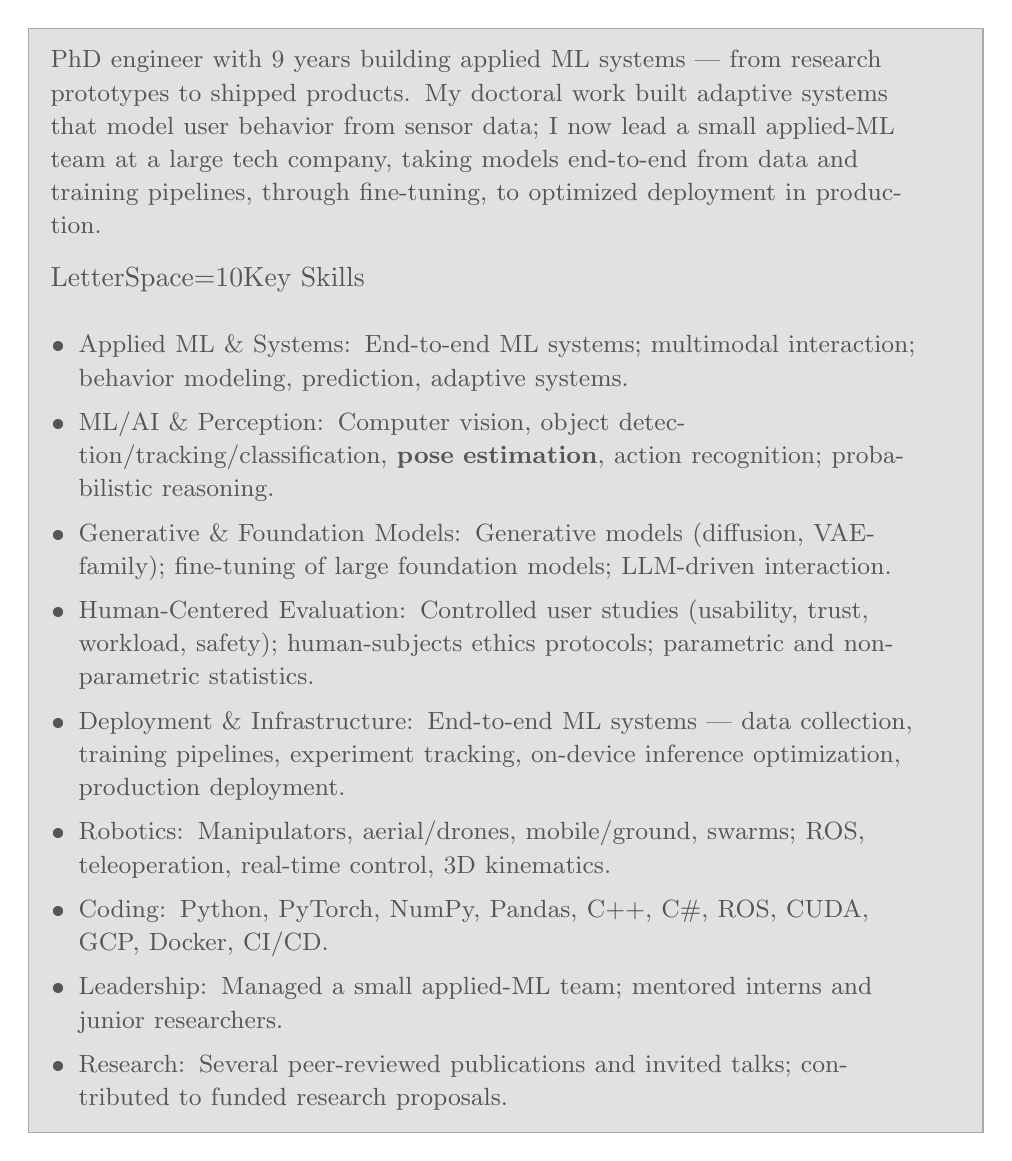
\begin{tikzpicture}
\node[draw=boxborder, line width=0.5pt, fill=boxbg, inner sep=8pt, text width=\dimexpr\textwidth-16pt\relax, align=left] {%
\begin{minipage}{\dimexpr\textwidth-16pt\relax}
\color{darkgrey}{\profileFont
PhD engineer with \textmedium{9 years building applied ML systems} --- from research prototypes to shipped products. My doctoral work built adaptive systems that model user behavior from sensor data; I now lead a small applied-ML team at a large tech company, taking models end-to-end from data and training pipelines, through fine-tuning, to optimized deployment in production.
}\\[7pt]
{\keySkillsTitleFont Key Skills}\\[0pt]
\color{darkgrey}{\keySkillsBulletFont
\begin{itemize}[leftmargin=1.1em, itemsep=0pt, topsep=0pt]
\item \textmedium{Applied ML \& Systems:} End-to-end ML systems; multimodal interaction; behavior modeling, prediction, adaptive systems.
\item \textmedium{ML/AI \& Perception:} Computer vision, object detection/tracking/classification, \textbf{pose estimation}, action recognition; probabilistic reasoning.
\item \textmedium{Generative \& Foundation Models:} Generative models (diffusion, VAE-family); fine-tuning of large foundation models; LLM-driven interaction.
\item \textmedium{Human-Centered Evaluation:} Controlled user studies (usability, trust, workload, safety); human-subjects ethics protocols; parametric and non-parametric statistics.
\item \textmedium{Deployment \& Infrastructure:} End-to-end ML systems --- data collection, training pipelines, experiment tracking, on-device inference optimization, production deployment.
\item \textmedium{Robotics:} Manipulators, aerial/drones, mobile/ground, swarms; ROS, teleoperation, real-time control, 3D kinematics.
\item \textmedium{Coding:} Python, PyTorch, NumPy, Pandas, C++, C\#, ROS, CUDA, GCP, Docker, CI/CD.
\item \textmedium{Leadership:} Managed a small applied-ML team; mentored interns and junior researchers.
\item \textmedium{Research:} Several peer-reviewed publications and invited talks; contributed to funded research proposals.
\end{itemize}
}
\end{minipage}
};
\end{tikzpicture}

\vspace{14pt}

% ═══════════════════ WORK EXPERIENCE ═══════════════════
% MASTER: superset of impact bullets per role. Keep the most role-relevant, cut the rest.
\sectitle{Work Experience}

{\dateFont Sep 2024 - present}\\[1pt]
{\boldHeadFont Company A (City, Country)}\hspace{10pt}{\italicHeadFont ML/AI Engineer - Applied ML Team}\\[-.3cm]
{\jobBulletFont
\begin{itemize}
\item Leading initiatives on \textbf{embodied agents} and \textbf{tracking systems} for real-world deployment.
\item Building \textbf{multimodal interaction} combining \textbf{multiple sensor modalities}.
\item Designing and implementing \textbf{user-facing behavior} across a consumer product.
\item Generating \textbf{synthetic motion} with \textbf{diffusion and VAE-family} models.
\item Shipped an \textbf{\cvlink{https://example.com}{open-source sample}} (example date): \textbf{perception}, \textbf{foundation model}, \textbf{60 fps} tracking.
\item Fine-tuned \textbf{foundation models} on a large motion dataset for real-time applications.
\item Shipped \textbf{tracking features} for a flagship product --- \textbf{ships in every unit, 60 fps}.
\item Evaluating interaction \textbf{usability, trust, and safety} through structured \textbf{user studies}.
\item Driving research and production in \textbf{pose estimation}, \textbf{motion prediction}, and \textbf{sensor fusion}.
\item Setting \textbf{technical direction} and mentoring engineers across research, engineering, and product teams.
\end{itemize}
}

\vspace{7pt}
{\dateFont Sep 2021 - Sep 2024}\\[1pt]
{\boldHeadFont Company B (City, Country)}\hspace{10pt}{\italicHeadFont Staff ML/AI Engineer \& Sr. Manager - Applied Team}\\[-.3cm]
{\jobBulletFont
\begin{itemize}
\item Led a \textbf{small engineering team} building a product feature, deployed across \textbf{thousands of devices}.
\item Built \textbf{object detection, tracking}, \textbf{gesture classification}, and \textbf{action recognition} at \textbf{60 fps on-device}.
\item \textbf{Productized} key AI/ML technologies into \textbf{platform capabilities adopted cross-company}.
\item Owned the \textbf{software stack} across engine/language, networking, animation, and a data pipeline; experiment tracking and inference optimization.
\item Helped define \textbf{strategic direction and roadmap} for the initiative with leadership.
\item \textbf{Mentored interns} and drove alignment across research, engineering, product, and design teams.
\end{itemize}
}

\vspace{7pt}
{\dateFont Jul 2017 - Sep 2021}\\[1pt]
{\boldHeadFont University X (City, Country)}\hspace{10pt}{\italicHeadFont Doctoral researcher - Machine Learning}\\[-.3cm]
{\jobBulletFont
\begin{itemize}
\item Developed ML models for \textbf{behavior understanding}, \textbf{intent recognition}, and \textbf{trajectory prediction}.
\item Designed and evaluated \textbf{personalized interfaces} for robotic platforms.
\item Built \textbf{online-adaptive models} classifying sensor signals to infer \textbf{user intent} in real time.
\item Ran \textbf{several controlled user studies} on usability, trust, and workload under human-subjects ethics approval.
\item Published \textbf{several first-author papers}; contributed to funded research proposals.
\item Teaching assistant in several master courses; supervised student projects; international collaborations.
\end{itemize}
}
\vspace{2pt}
{\refFont
Ref: Prof. Jane Advisor (\underline{\href{mailto:advisor@example.edu}{advisor@example.edu}}),
Dr. Sam Collaborator (\underline{\href{mailto:collaborator@example.com}{collaborator@example.com}})
}

\vspace{7pt}
{\dateFont Jul 2015 - Sep 2017}\\[1pt]
{\boldHeadFont Research Lab Y (City, Country)}\hspace{10pt}{\italicHeadFont Data Analyst and Lab Coordinator}\\[-.3cm]
{\jobBulletFont
\begin{itemize}
\item Built \textbf{automated data-analysis software} reprocessing the full sample database, \textbf{cutting manual analysis $\sim$50\%}.
\item Enabled real-time tuning at a higher sample throughput; drove experiment scheduling from analysis.
\item Commissioned, tested, and installed \textbf{lab equipment}; built the \textbf{acquisition and control system}.
\end{itemize}
}
\vspace{2pt}
{\refFont
Ref: Dr. Alex Mentor (\underline{\href{mailto:mentor@example.org}{mentor@example.org}})
}

\vspace{5pt}

\newpage

% ═══════════════════ EDUCATION ═══════════════════
\sectitle{Education}

{\boldHeadFont Ph.D. in Robotics, \cvlink{https://example.edu}{with Distinction}} --- {\instituteFont University X (City, Country); example ranking note}\\
{\thesisFont \underline{Thesis}:\ Example thesis title about adaptive interfaces for robot control. \emph{Recipient, example best-thesis award.}}

\vspace{10pt}
{\boldHeadFont Master of Science in Automation and Robotic Engineering}\\
{\instituteFont University Z (City, Country)}\\
{\thesisFont \underline{Thesis}:\ Example thesis title about motion control design}

\vspace{10pt}
{\boldHeadFont Bachelor's degree in Electronic Engineering}\\
{\instituteFont University Z (City, Country)}\\
{\thesisFont \underline{Thesis}:\ Example thesis title about signal processing for distance sensors}

\vspace{14pt}

% ═══════════════════ TECHNICAL SKILLS ═══════════════════
% MASTER: every category. Cut/merge per role (original base used Programming/Data/3D-XR/More).
\sectitle{Technical skills}

\vspace{5pt}
\skilltitle{Human-Robot Interaction \& Evaluation}
\vspace{-4pt}
{\bulletFont
\begin{itemize}
\item Multimodal interaction \textbf{(speech/voice, gesture, gaze \& eye tracking, posture, proxemics)}
\item Affective computing, social signal processing; human intent recognition, prediction, adaptive behavior generation
\item User studies \textbf{(experiment design, usability / trust / workload evaluation, human-subjects ethics protocols)}
\item Statistical models \textbf{(normal: t-test, F-test, ANOVA, non-normal: Mann Whitney, Kruskal-Wallis, Levene…)}
\end{itemize}
}

\vspace{5pt}
\skilltitle{Robotics \& Embodied AI}
\vspace{-4pt}
{\bulletFont
\begin{itemize}
\item Platforms \textbf{(robotic hands, manipulators, mobile/ground, aerial/drones, multi-robot swarms)}
\item Digital humans and embodied agents \textbf{(avatars, socially situated behavior, hand and full-body control)}
\item ROS, teleoperation, real-time control, sensor fusion
\item 3D math \textbf{(rotation matrices, quaternions, Euler angles, direct/inverse kinematics, Jacobians)}
\item Body Motion Capture Systems +\ processing \textbf{(OptiTrack/Motive, XR Devices, Leap Motion, EMG, IMUs)}
\end{itemize}
}

\vspace{5pt}
\skilltitle{AI / ML \& Perception}
\vspace{-4pt}
{\bulletFont
\begin{itemize}
\item Frameworks and tools \textbf{(PyTorch, SKLearn, Numpy, Pandas, Matplotlib, IPython, CUDA)}
\item Computer vision \textbf{(object detection, tracking, classification, pose estimation, action recognition)}
\item Sequence learning, motion and intent prediction, sensor fusion; probabilistic and Bayesian reasoning
\item Natural language processing \textbf{(NLP)}; digital signal processing \textbf{(FFT, time-frequency analysis, system identification)}
\end{itemize}
}

\vspace{5pt}
\skilltitle{Foundation Models \& Deployment}
\vspace{-4pt}
{\bulletFont
\begin{itemize}
\item Foundation models \textbf{(fine-tuning and deployment; Gemini/Gemma; LLM-driven interaction and agents)}
\item End-to-end ML systems \textbf{(data collection $\rightarrow$ training pipelines $\rightarrow$ on-device deployment)}
\item Training pipelines, experiment tracking, tooling for fast model iteration across teams
\item Inference optimization under latency budgets; GPU-accelerated training \textbf{(PyTorch/CUDA)}
\end{itemize}
}

\vspace{5pt}
\skilltitle{Programming \& Infrastructure}
\vspace{-4pt}
{\bulletFont
\begin{itemize}
\item Programming languages and tools - excellent knowledge \textbf{(C++, C\#, Python, ROS, Matlab/Simulink)}
\item Programming languages - good knowledge \textbf{(LabVIEW, VHDL)}
\item Version control, Issue tracking, cloud computing, virtualization \textbf{(GIT,\ CI/CD, Jira, GCP, Docker…)}
\item Firmware/Embedded Software development \textbf{(Arduino, STM32F4, BeagleBone, Raspberry Pi, Cypress PSOC)}
\end{itemize}
}

\vspace{5pt}
\skilltitle{3D / XR}
\vspace{-4pt}
{\bulletFont
\begin{itemize}
\item VR/XR application development \textbf{(Unity3D, Blender, Android XR, OpenXR)}
\item Skeletal animation, blendshapes, rigging, 3D modeling
\end{itemize}
}

\vspace{14pt}

% ═══════════════════ LANGUAGE SKILLS ═══════════════════
\sectitle{Language Skills}
\vspace{4pt}

{\subtitleFont
$\hspace{5pt}\bullet$\ \hspace{4pt}\textbf{Italian} - Native
\hspace{14pt}$\bullet$\ \hspace{4pt}\textbf{English} - Fluent (C1)
\hspace{14pt}$\bullet$\ \hspace{4pt}\textbf{French} - Fluent (B2)
\hspace{14pt}$\bullet$\ \hspace{4pt}\textbf{German} - Basic (A1)
}

\vspace{14pt}

% ═══════════════════ TRAINING & CERTS ═══════════════════
\sectitle{Advanced training and certifications}

{\bulletFont
\begin{itemize}
\item \avenirmedium{Neural Networks and Deep Learning specialization} \avenir{(2022, by Coursera)}
\item \avenirmedium{PRINCE2 2017 Project Management Certification} \avenir(2020, by Axelos Global Best Practice)
\item \avenirmedium{Start-Up Training - Business Concept} \avenir(2019, by INNOSUISSE - Swiss Innovation Agency)
\item \avenirmedium{International School on Human Body Motion} \avenir(2017, Heidelberg)
\item \avenirmedium{Certified LabVIEW Associate Developer - CLAD} \avenir(2016, by National Instruments)
\item \avenirmedium{FPGA Design Using VHDL - Advanced} \avenir(2015, by Doulos)
\end{itemize}
}

\vspace{14pt}

% ═══════════════════ HONORS & AWARDS ═══════════════════
\sectitle{Honors \& Awards}

{\bulletFont
\begin{itemize}
\item \avenirmedium \cvlink{https://example.edu}{Best PhD Thesis Award} (University X, example year)
\item \avenirmedium \cvlink{https://example.org}{Technical Student Scholarship} (Research Lab Y, example year)
\item \avenirmedium \cvlink{https://example.edu}{Top 1\% student placement test} (University Z, example year)
\item \avenirmedium {National finalist of the national Mathematical Olympiad} (2007)
\end{itemize}
}

\vspace{14pt}

% ═══════════════════ EXTRACURRICULAR ═══════════════════
\sectitle{Extracurricular activities}

{\bulletFont
\begin{itemize}
\item Passionate in reading and writing, good writing ability (technical and creative)
\item Passionate in tennis, golf, boxing, piano
\item National chess finalist
\end{itemize}
}

\newpage

% ═══════════════════ SCIENTIFIC ACTIVITIES ═══════════════════
\sectitle{Scientific Activities}

\vspace{4pt}
{\subtitleBoldFont Selected Publications}\ \ {\refFont example: also featured at a major conference}

\vspace{6pt}
{\bulletFont
\begin{itemize}[itemsep=2pt]
\item \textbf{J. Candidate}, A. Coauthor, B. Coauthor, C. Coauthor,
\textbf{"Example paper title about adaptive interface classification"},
Example Journal, \underline{IN REVIEW}
\item \textbf{J. Candidate}, A. Coauthor, B. Coauthor,
\textbf{"Example paper title about data-driven personalization"},
Example Journal, \underline{IN REVIEW}
\item \textbf{J. Candidate}, A. Coauthor, B. Coauthor,
\textbf{"Example paper title about fast machine learning of interfaces"}
Example Robotics Letters (2019)
\item \textbf{J. Candidate}, A. Coauthor, B. Coauthor,
\textmedium{"Example paper title about a fitness study of interface design"}
- Example Conference on Human Interaction (2021).
\item \textbf{J. Candidate}, A. Coauthor, B. Coauthor,
\textbf{"Example paper title about personalized swarm interaction"}
(2021) - Example Robotics Letters
\item \textbf{J. Candidate}, A. Coauthor, B. Coauthor,
\textbf{"Example paper title about a haptic teleoperation interface."}
Example Intl. Conf. Robotics Automation (2020).
\item \textbf{J. Candidate}, A. Coauthor, B. Coauthor,
\textbf{"Example paper title about VR viewpoints in teleoperation"}
- Example VR Conference (2021)
\item A. Coauthor, B. Coauthor, C. Coauthor, and \textbf{J. Candidate}.
\textmedium{"Example paper title about a measurement instrument control system."},
Example Control Conference (2017)
\item A. Coauthor, B. Coauthor, \textbf{J. Candidate}, C. Coauthor,
\textmedium{"Example paper title about applied engineering."},
Example Trans. Appl. (2016)
\end{itemize}
}

\vspace{6pt}
{\subtitleBoldFont Oral Presentations \& Invited Talks}

\vspace{6pt}
{\bulletFont
\begin{itemize}[itemsep=5pt]
\item \textbf{Example Conference 2021}, \emph{"Example talk title about adaptive interfaces."} (online, 2021)
\item \textbf{Example VR Conference 2021}, \emph{"Example talk title about VR viewpoints in teleoperation."} (City - online, 2021)
\item \textbf{Example ICRA 2020}, \emph{"Example talk title about a haptic teleoperation interface."} (City - online, 2020)
\item \textbf{Example Symposium 2018,} \emph{"Example talk title about motion-based piloting."} (City, 2018)
\item \textbf{Example Workshop 2018,} \emph{"Example talk title about motion as a data source."} (City, 2017)
\end{itemize}
}

\end{document}
